%---------------------------------------------------------------------------------------------------
% Hauptteil
%---------------------------------------------------------------------------------------------------
%\newpage
%%\part{Hauptteil}

% Kapitel 1: Von der Integration zur Inklusion - eine Begriffserkl�rung 
\chapter{Organisationsstruktur}
  \section{Arbeitsfeldbeschreibung}\label{sec:2_1}
    \begin{flushleft}
      Die Kindertagesst�tte der Gemeinde Oststeinbek mit sechs Elementargruppen, einer Integrationsgruppe und sechs weiteren Hortgruppen, liegt gesch�tzt im Forellenbachpark im Kreis Stormarn, fernab vom Stra�enverkehr und grenzt r�umlich direkt an die Grundschule an. So beherbergt diese Einrichtung von Montag bis Freitag von 7:00 - 17:00 Uhr ca. 210 Kindern im Alter von drei bis vierzehn Jahren.\citep[vgl.][]{oststein2013}
    \end{flushleft}

    \begin{flushleft}
      Anf�nglich wurde die Einrichtung alleine von Herrn Strau� geleitet, dies �nderte sich mit dem erh�hten Bedarf au�erfamili�rer Betreuung. So hat sich dieser in den letzten 10 Jahren mehr als verdoppelt. Daher wurde entschieden, dass die Kita und der Hort zwar weiterhin eng zusammenarbeiten, aber nun mehr von zwei verschiedenen Personen geleitet werden. Die Leitung der Kita wird weiterhin von Herrn Strau� �bernommen und Frau Peters tut dies nun  f�r den angrenzenden Hort. Da der Bedarf immer noch sehr hoch ist, unteranderem auch durch die gesetzliche �nderung f�r die Betreuung von unter Dreij�hrigen, und der Einrichtung keinerlei r�umliche Kapazit�ten mehr zur Verf�gung stehen, wird auf dem Nachbargel�nde ein weiteres Kita-Geb�ude gebaut.
    \end{flushleft}

  \newpage
  \section{Aufgabenbeschreibung}\label{sec:2_2}
    \begin{flushleft}
      Die Kindertagesst�tte ist wie ein kleines Unternehmen, dass die Kita-Leitungskraft- in meinem Fall Herr Strau�- f�hrt. Daher sind die Aufgaben, die er bew�ltigen muss, sehr vielf�ltig. Das Organisieren und Managen dieses Unternehmens nimmt einen gro�en Teil seiner Arbeit ein. Hier bei versucht er immer die p�dagogischen, personellen und betriebswirtschaftlichen Aspekten im Auge zu behalten.\citep[vgl.][]{elbkind2013}
    \end{flushleft}

    \begin{flushleft}
      Auf Grund dessen geh�rt es zu seinen Aufgaben, die p�dagogischen Fachkr�fte zu unterst�tzen, ihnen beratend zur Seite zu stehen und sie gegebenfalls auch anzuleiten. Au�erdem liegt ihm die F�rderung seiner Mitarbeiter sehr am Herzen. In regelm��ig stattfindenden Mitarbeitergespr�chen, formulieren beide ein unabh�ngiges und ein gemeinsames Ziel f�r den Mitarbeiter. Nach einem ca. einem Jahr wird geguckt  inwieweit der P�dagoge sein und das gemeinsame Ziel erreicht hat und was er gegeben falls noch ben�tigt, um dies umsetzen zu k�nnen. Mit dieser Ma�nahmen versucht Herr Strau� die Qualit�t der p�dagogischen Arbeit bei einem hohen Niveau zu halten. Dabei ist ihm wichtig einen kooperativen F�hrungsstil zu pflegen, sodass die p�dagogischen Fachkr�fte einen gewissen p�dagogischen Freiraum haben. Dies geschieht aber immer in Anlehnung an das Konzept der Kita, das in Zusammenarbeit aller Mitarbeiter immer wieder modifiziert wird.\citep[vgl.][]{elbkind2013}
    \end{flushleft}



    \begin{flushleft}
      Da die Elternarbeit einen bedeutenden Teil der p�dagogischen Arbeit ausmacht, ist es Herrn Strau�  wichtig, dass seine Mitarbeiter die partnerschaftliche Zusammenarbeit mit den Eltern wahrnehmen und ber�cksichtigen. Zudem steht er den Eltern und dem p�dagogischen Fachpersonal bei gravierenden Problemen, wie zum Beispiel bei Entwicklungsschwierigkeiten des  Kindes, beratend zur Seite. Herr Strau� vermittelt die Eltern gegebenfalls an andere Institutionen und guckt mit ihnen inwieweit die Kita einen Beitrag dazu leisten kann.\citep[vgl.][]{elbkind2013}
    \end{flushleft}

    \begin{flushleft}
      Als Kita-Leitungskraft ist Herr Strau� au�erdem das Bindeglied - er bezeichnet es auch gerne als Sandwichsystem- zwischen der Kindertagesst�tte und dem Tr�ger. Unteranderem arbeitet er hier eng mit der Fachbereichsleitung zusammen und nimmt an unterschiedlichen Planungs- und Entscheidungsprozessen des Tr�gers teil. Derzeitig wird stark diskutiert und geplant wie man dem ver�nderten Betreuungsanspruch f�r unter Dreij�hrige gerecht werden kann.\citep[vgl.][]{elbkind2013}
    \end{flushleft}

    \begin{flushleft}
      Auch wenn Herr Strau� als Bindeglied zwischen dem Tr�ger (die Gemeinde Oststeinbek) und der Kita fungiert, muss er vieles eigenverantwortlich l�sen. Dazu geh�rt es neues Personal einzustellen, die Dienstpl�ne zu erstellen, sich mit politischen Ereignissen auseinanderzusetzen und mit den finanziellen Ressourcen f�r die Kita wirtschaftlich zu planen und entscheiden. Durch den administrativen Part, ist er seit vielen Jahren auf den PC angewiesen. Diese Arbeit erledigt er dienstags meist im Rathaus, da er dort die M�glichkeit hat ungest�rt zu arbeiten. \citep[vgl.][]{elbkind2013}
    \end{flushleft}
  
  \section{Rechtliche Grundlage}\label{sec:2_3}
    \begin{flushleft}
      Die Kindertagesst�tte Oststeinbek muss sich rein rechtlich an die auf Landes- und Bundesebene geltenden Gesetzte halten. Die rechtliche Grundlage, f�r Tageseinrichtungen in gesamt Deutschland, bildet das SGB VIII. Des Weiteren spielen das Kindertagesst�ttengesetz (KiTaG) und der Jugendhilfe-Rahmenvertrag f�r Schleswig-Holstein eine wichtige Rolle. Ich werde auf einige f�r die Kindertagespflege wichtigen gesetzlichen Richtlinien eingehen und sie erkl�ren.
    \end{flushleft}

    \subsection{Bundesebene: Sozialgestztbuch (SGB) Achtes Buch VIII -Kinder und Jugendhilfe-}\label{sec:2_3_1}
      \begin{flushleft}
        Entstanden ist das SGB VIII aus dem Kinder- und Jugendhilfegesetz (KJHG). Dies war wiederum an die Stelle des Jugenswohlfahrtgesetz ger�ckt. Seit dem Inkrafttreten des Gesetzes (1.1.1991) gab es schon viele Ver�nderungen. (SGB VIII Auf. 7 S. 11) Die derzeitig entscheidenden Ver�nderungen f�r die Kita- Landschaft sind die Ver�nderungen und Erweiterungen der �24 und �24a.
      \end{flushleft}

      \begin{flushleft}
        Organisiert wird die F�rderung von Kindern in Tageseinrichtungen und in der Kindertagespflege in den �� 22 bis 26  SGB VIII. Die Grunds�tze der F�rderung in Kindertageseinrichtungen werden im � 22 geregelt. Nach � 22 Abs.1 SGB VIII sind Tageseinrichtungen Einrichtungen, in denen sich Kinder f�r einen Teil des Tages oder ganzt�gig aufhalten und in Gruppen gef�rdert werden. Im zweiten Absatz dieses Paragraphen wird erl�utert welchen Auftrag die Kindertagespflege hat. Dieser ist zum einen die Entwicklung der Kinder zu eigenverantwortlichen und gemeinschaftlichen Pers�nlichkeiten zu f�rdern, sowie zum anderen die Erziehung und Bildung in der Familie zu unterst�tzen und erg�nzen. Au�erdem besteht der Auftrag der Tageseinrichtung darin, den Eltern dabei zu  helfen, ihre Erwerbst�tigkeit und Kindererziehung besser miteinander vereinbaren zu k�nnen. Um den F�rderungsauftrag von Kindertageseinrichtungen geht es in � 22 Abs. 3. Dieser umfasst die  Erziehung, Bildung und Betreuung von Kindern und bezieht sich auf die soziale, emotionale, k�rperliche und geistige Entwicklung von Kindern. Des Weiteren wird im � 22a auf die F�rderung in Tageseinrichtungen eingegangen. So ist dort geschrieben, dass die Tr�ger der �ffentlichen Jugendhilfe (siehe SGB VIII � 69) die Qualit�t der F�rderung in ihren Einrichtungen durch eigene Ma�nahmen sicherstellen und weiterentwickeln sollen. Ein ebenfalls wichtiger Paragraph f�r die Arbeit in Kindertageseinrichtungen ist der  � 24. Dieser hat gerade durch den aktuellen Diskurs und seine entscheidenden Ver�nderungen, die am 1.8.2013 in Kraft getreten sind, an Aufmerksamkeit gewonnen. So wurde der � 24 im Zuge des Ausbaus der Kinderbetreuung dahingehend erweitert und ver�ndert, dass Kinder die das erste Lebensjahr noch nicht vollendet haben unter bestimmten Voraussetzungen in einer Tageseinrichtung oder Kindertagespflege gef�rdert werden. Somit haben entsprechende Kinder, ab den ersten Lebensjahr bis Vollendung des dritten Lebensjahres einen Anspruch auf au�erfamil�re fr�hkindliche F�rderung. Nun stehen die Tr�ger und Kitas in der Pflicht dies m�glich zu machen. Bestehen bleibt das Gesetz das Kinder vom dritten Lebensjahr bis zum Schuleintritt ein Recht auf den Besuch einer Kindertageseinrichtung haben.\citep[vgl.][S.~24]{SGBVIII2012}
      \end{flushleft}

      \begin{flushleft}
        Als Leitung einer Kindertagesst�tte sind weiter Gesetzte aus dem Sozial Gesetzb�chern von Bedeutung. So ist die Betriebserlaubnis von Kitas im � 45 SGB VIII geregelt und bei Unf�llen in der Kindertagesst�tte, in Begleitung einer p�dagogischen Fachkraft der Einrichtung und auf dem Weg von und zur Einrichtung sind die Kinder gesetzlich versichert, dies ist im �2 Abs. 1 Nr. 8 des SGB VII geregelt.\citep[vgl.][S.~26]{SGBVIII2012} 
      \end{flushleft}
      
      \begin{flushleft}
        Um einen l�ckenlosen Schutz vor einer Kindeswohlgef�hrdung zu gew�hren sind Tr�ger, Kita-Leitung und das p�dagogische Fachpersonal durch den � 8a Abs. 4 SGB VIII dazu angehalten bei der Annahme einer Gef�hrdung des Kindeswohls dem nach zu gehen. So haben Fachkr�fte die Aufgaben gewichtige Anhaltspunkte zu dokumentieren und einzusch�tzen. Im weiteren Verlauf haben sie erfahrenere Kr�fte hinzuzuziehen, die Betroffenen mit einzubeziehen und ihnen Hilfe anzubieten. Wenn die angenommene Hilfe nicht ausreicht, ist das Jugendamt mit einzubeziehen
      \end{flushleft}

    \newpage
    \subsection{Landesebene: Gesetz zur F"orderung von Kindern in Tageseinrichtungen und Tagespflegestellen (Kindertagesst"attengesetz - KiTaG)}\label{sec:2_3_2}
      \begin{flushleft}
        Da die Kindertagesst�tte Oststeinbek sich im Bundesland Schleswig-Holstein befindet, haben Tr�ger, Kita-Leitung und das p�dagogische Fachpersonal sich nach den gesetzlichen Richtlinien f�r dieses Bundesland zu richten. Zum einen gilt hier das Kindertagesst�ttengesetz - KiTaG und zum anderen das Kindertagesst�tten- und -tagespflegeverordnung - KiTaVO. Das KiTa G dient zur Ausf�hrung der Regelungen zur F�rderung von Kindern in Kindertageseinrichtungen und Tagespflege nach den �� 22 bis 26 SGB VIII. Aus diesem Grund unterscheidet es sich kaum von dem bundesweiten Bestimmungen f�r das Kita-Wesen. Einige der Punkte wurden erweitert oder komplett �bernommen. {KiTaG2013} Das KiTaVO wiederum regelt, seit dem 13. November 1992, die Mindestanforderungen f�r den Betrieb von Kindertages- einrichtungen und f�r die Leistungen, die von der Kindertagespflege erbracht werden sollen. \citep[vgl.][]{KiTaVO2013}
      \end{flushleft}

      \begin{flushleft}
        Ebenfalls von Bedeutung f�r Kindertageseinrichtungen in Schleswig-Holstein ist der Jugendhilfe-Rahmenvertrag. Dieser wurde am 16. Februar 2009 gem�� � 78f SGB VIII die kommunalen Spitzenverb�nde mit den Verb�nden und Tr�gern von Einrichtungen nach � 78f SGB VIII geschlossen. Der Vertrag regelt die Rahmenbedingungen f�r Leistungs-, Entgelt- und Qualit�tsentwicklungsvereinbarungen nach � 78b SGB VIII. \citep[vgl.][]{JugendhR2013}
      \end{flushleft}
  \newpage
  \section{Darlegung der gew"ahlten Methoden und Instrumente Beschreibung der Ergebnisse }\label{sec:2_4}
    \begin{flushleft}
      Um einen authentischen Blick auf die Arbeit einer Kita-Leitungskraft zu bekommen, habe ich ein Shadowing und ein Interview -siehe Anhang- durchgef�hrt. Beide Dinge haben mir einen guten ein Blick in das Berufsfeld einer Kita-Leitungskraft gegeben. Beim Shadowing durfte ich Herrn Strau� einen ganzen Arbeitstag folgen und war im wahrsten Sinne des Wortes sein Schatten. Hierbei konnte ich beobachten wie der Arbeitsalltag einer Kita-Leitung aussieht. Beim Beschatten ist mir aufgefallen wie abwechslungsreich und vielf�ltig dieser Alltag ist. Der regul�re Arbeitsbeginn von Herrn Strau� ist um 8:00 Uhr morgens. Er kommt ca. 10 bis 15 Minuten fr�her um sich erst einmal einzurichten. Eine seiner ersten Amtshandlungen ist es sich insoweit f�r das zu organisieren, was f�r ihn an diesem Tag anliegt. In diesem Zeitraum kommen immer wieder Eltern und Mitarbeiter mit Anliegen zu ihm. Um alle Mitarbeiter zu begr��en, sich nach ihren Befindlichkeiten zu erkundigen und sie �ber wichtige Ereignisse zu informieren, wird sich kurz, im Fr�hdienstbereich der Kita, getroffen. Nach dem Austausch, geht Herr Strau� durchs Haus, um den Eltern eine gewisse Pr�senz zu vermitteln. Anschlie�end folgen einige Telefonate, nebenbei sortiert er die Postmappe die ans Rathaus gehen soll und schreibt einen Aushang f�r die Eltern. Zudem steht er Eltern und Mitarbeitern mit Rat und Tat zur Seite. Hierzu geh�ren auch Elternrumf�hrungen, bei denen er  Eltern, die an einem Kitaplatz Interesse haben, zeigt wie die Kita und deren Alltag gestaltet sind. Da Herr Strau� administrative Angelegenheiten dienstags ganzt�gig und den Rest der Woche immer ab 13 Uhr erledigt, versucht er wichtige Gespr�che in den Vormittagsbereich zu legen. An dem Tag des Shadowings war dies auch der Fall, so hatte er ein Gespr�ch mit der Hort - und der Fachbereichsleitung, �ber den Ausbau der Kita.
    \end{flushleft}

    \begin{flushleft}
      Das Interview wiederum hat mir vor Augen gef�hrt, was eine Kita-Leitung braucht um diesen anspruchsvollen T�tigkeit gerecht zu werden. Zum einen w�re da die Ausbildung bzw. das Studium, das theoretisches Wissen �ber die p�dagogische Arbeit vermittelt. Zum anderen sind da die F�higkeiten, die im Laufe der Berufst�tigkeit erworben und erweitert werden. Dazu geh�ren unteranderem der administrative Part, zu erkennen was wichtig und was unwichtig ist, ein vern�nftiges Zeitmanagement zu haben und einen angemessenen Umgang mit Eltern zu pflegen.
    \end{flushleft}



\newpage

% Kapitel 2: Fehldeutungen und Chancen von Inklusion				
\chapter{Auswertung, B"undelung und Interpretation der Ergebnisse}\label{sec:3}
  \section{Zentrale Kompetenzbereiche}\label{sec:3_1}
    \begin{flushleft}
      Die vielf�ltigen und hoch komplexen Aufgaben und die nicht Vorhersehbarkeit des fr�hp�dagogischen Alltags verlangt einer Kita-Leitungskraft  umfassende Kompetenzen ab. Gerade durch den derzeitigen Diskurs in der Fach�ffentlichkeit hat der Kompetenzbegriff an Bedeutung gewonnen. Der Erwerb von Kompetenzen sollte f�r die Kita-Leitungskraft und das p�dagogische Fachpersonal einen �bergeordnetes Ziel sein. Ihre Aufgabe ist es Fachwissen Erfahrungswissen, F�higkeiten und Fertigkeiten in den komplexen Situationen zu reflektieren und organisiert aktuellen Anforderungen zu begegnen und Probleme zu l�sen. Die Hauptkompetenz ist die Handlungskompetenz, die sich in vier Teildimensionen klassifizieren l�sst.\citep[vgl.][S.~17f]{Kompet2011} 
    \end{flushleft}

    \begin{center}
      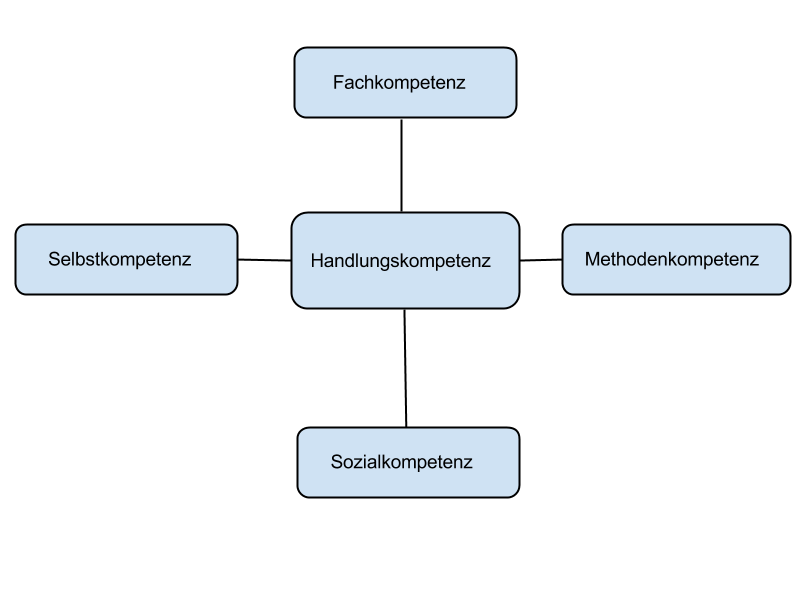
\includegraphics[width=1.0\textwidth]{grafik/taetigkeitspr.png}
      \captionof{figure}[Vierdimensionales Kompetenzmodell]{Vierdimensionales Kompetenzmodell \citep[vgl.][S.~15]{Kompet2011}}
      \label{fig:zusammenhang}
    \end{center}

    \begin{flushleft}
      Zum einen w�re da die Fachkompetenz. So braucht eine Kita-Leitung p�dagogisches Fachwissen, politisches Wissen, Wissen �ber den gesetzlichen Rahmen und EDV Kenntnisse, um den komplexen Situationen auf fachlicher Ebene entgegen treten zu k�nnen. \citep[vgl.][S.~11]{Fuhr2012} 
    \end{flushleft}

    \begin{flushleft}
      Im Bereich der Methodenkompetenz geht es darum, durch die Anwendung von Methoden und Techniken Dinge oder Situationen zu planen und organisieren, um am Ende ein bestimmtes Ziele zu erreichen. Im Fall der Kita-Leitungskraft hei�t das z.B. die F�higkeit zu haben, auf Fragen oder Anliegen von Eltern oder dem p�dagogischen Fachpersonals angemessen und fachgerecht zu antworten und helfen zu k�nnen. Das hei�t nicht, dass sie alles wissen muss, aber sie sollte wissen wo sie nachzuschlagen hat. \citep[vgl.][S.~12]{Fuhr2012} 
    \end{flushleft}

    \begin{flushleft}
      Das Ziel einer Leitungskraft ist es, dass das Team gut zusammenarbeitet  und die Beziehung zu den Eltern auf gegenseitigen Respekt beruht, um dem gemeinsamen Hauptziel, die Kinder gemeinsam zu bilden und zu erziehen, gerecht zu werden. Damit dies gelingt, wird einer Kita-Leitung eine Vielfalt an sozialen Kompetenzen wie Einf�hlungsverm�gen, Kommunikationstalent, Teamf�higkeit, Konfliktbereitschaft, Empathie, Flexibilit�t, Offenheit und viele weitere Soft Skills abverlangt. So ist Anerkennung f�r getane Leistung genauso wichtig, wie auch konstruktive Kritik aussprechen zu k�nnen. \citep[vgl.][S.~12]{Fuhr2012} 
    \end{flushleft}

    \begin{flushleft}
      Durch die Komplexit�t der F�hrungsposition und die hohen Verantwortungen, die eine Kita-Leitung zu tragen hat, ist ihr Terminkalender immer gef�llt. Um den verschiedenen Anforderungen entsprechend reagieren zu k�nnen, ben�tigt sie ein hohes Ma� an Selbstkompetenz. Dies umfasst unteranderen die pers�nliche Belastbarkeit, die pers�nliche Arbeitsorganisation und  das Zeitmanagement. Wer f�r sich wichtiges von unwichtigen unterscheiden kann, wei� wo er Priorit�ten setzen kann. \citep[vgl.][S.~13]{Fuhr2012}
    \end{flushleft}


  \section{Organisationale Managementdimensionen}\label{sec:3_2}
    \begin{flushleft}
      Das Aufgabengebiet von Kita-Leitungskr�ften hat sich, in den letzten Jahren, dahingehend ver�ndert, dass der Bereich Management immer mehr an Bedeutung gewinnt und immer mehr in den Vordergrund r�ckt. Mitverantwortlich f�r das ver�nderte Aufgabengebiet, sind zum einen ver�nderte  Rahmenbedingungen und zum anderen die ver�nderten Bed�rfnisse der Eltern und Kinder. Um der Vielfalt an Aufgaben und Bed�rfnissen gerecht zu werden, ist es hilfreich die zehn verschiedenen Managementdimensionen (Organisations- und Dienstleistungsentwicklung, Konzeption und Konzeptionsentwicklung, Qualit�tsmanagement, Personalmanagement, Finanzmanagement, Familienorientierung und Elternbeteiligung, Gemeinwesenorientierte Vernetzung und Kooperation, Bedarfsermittlung und Angebotsplanung, �ffentlichkeitsarbeit, Bau und Sachausstattung) dabei zu beachten. Von gro�er Bedeutung ist es, in diesem Zusammenhang bedarfs- und marktgerecht sowie betriebswirtschaftlich zu denken und zu handeln. Dabei sollte das wichtigste Ziel sein, die drei Punkte Bildung, Erziehung Betreuung nicht aus den Augen zu verlieren. Im Folgenden wird darauf eingegangen, inwieweit die zehn organisationale Managementdimensionen eine Rolle f�r die Leitungskraft einer Kindertagesst�tte spielen. Hierbei werde ich mich auf Herrn Strau� und seine organisatorischen Aufgaben beziehen.
    \end{flushleft}

    \subsection{Organisations- und Dienstleistungsentwicklung}\label{sec:3_2_1}
      \begin{flushleft}
        Die Organisations- und Dienstleistungsentwicklung richtet sich nach dem Bedarf der Adressaten. Ein gutes Beispiel ist der Zuwachs, den Herr Strau� in seiner Arbeit als Kita-Leitung erlebt hat. Durch das Zuziehen von Familien und durch geburtenstarke Jahrg�nge, ist der Mehrbedarf an Betreuungspl�tzen in der Gemeinde Oststeinbek in den letzten 10 Jahren um mehr als das Doppelt gestiegen. Die Gemeinde als Tr�ger der Einrichtung und die Kita-Leitungen haben lange �berlegt wie sie dieser Ver�nderung begegnen k�nnen, da sowohl der Hort als auch die Kindertagesst�tte drohte aus allen N�hten zu platzen. So mussten und m�ssen sie erst einmal auf Alternativen ausweichen. Zu den Alternativen geh�rte unteranderem, dass sowohl der Hort als auch die Kita Au�enstellen errichten mussten. Die Gemeinde kaufte zwei leer stehende H�user und stellte zwei Container auf dem angrenzenden Schulgel�nde auf, um dem Zuwachs gerecht zu werden. Des Weiteren sind die Gruppen in den Hauptgeb�uden enger zusammen ger�ckt. Im Fr�hjahr 2014 soll der Bau des neuen Kitageb�udes abgeschlossen werden und die Lage soll sich bis dahin entspannen. \citep[vgl.][S.~23]{Trager2013}
      \end{flushleft}
      
    \subsection{Konzeption und Konzeptionsentwicklung}\label{sec:3_2_2}
      \begin{flushleft}
        Das Konzept ist ein wichtiger Baustein f�r jede Kindertagesst�tte, in dem festgehalten wird, wie sie dem Bildungs-, Betreuungs- und Erziehungsauftrages gerecht werden wollen. So hat die Kindertagesst�tte Oststeinbek unter anderem in ihrem Konzept stehen, dass sie nach dem Situationsansatz arbeiten, wie die Rolle des P�dagogen und der Eltern verstanden wird. Diese und weitere Dinge des Konzeptes werden in regelm��igen Abst�nden vom Kita-Team �berarbeitet und weiter entwickelt. Dabei setzen sie sich mit kontextuellen Ver�nderungen und situativen Anforderungen auseinander. Bedacht wird dabei auch immer der gesetzliche Rahmen. Herr Strau� hat hierbei zu koordinieren und zu organisieren wann dies geschieht. Zudem hat er darauf  Acht zu geben, dass alle Mitarbeiter nach diesem Konzept handeln. \citep[vgl.][S.~34]{Trager2013}
      \end{flushleft}
    
    \subsection{Qualit�tsmanagement}\label{sec:3_2_3}
      \begin{flushleft}
        Zum gro�en Managementsektor geh�rt es ebenfalls f�r Herrn Strau� als Kita-Leitungskraft dazu, die Qualit�t nicht au�er Acht zu lassen. Den Rahmen bilden f�r diese Einrichtung die Bildungsleitlinien des Bundeslandes Schleswig- Holstein und der nationale Kriterienkatalog. Die �berpr�fung der Qualit�t erfolgt durchs gesamte Team mit Hilfe des nationalen Kriterienkatalogs. \citep[vgl.][S.~47]{Trager2013}
      \end{flushleft}
      
    \subsection{Personalmanagement}\label{sec:3_2_4}
      \begin{flushleft}
        Des Weiteren geh�rt es zu den Aufgaben von Herrn Strau� das Personal zu organisieren und zu leiten. In diesem Zusammenhang guckt er wer eingestellt wird, wer welche Aufgaben im Team �bernimmt, ob alle Bildungbereiche vom Team abgedeckt werden, wer sich wie weiterbilden lassen kann und wer wie stark belastbar ist. Zudem erstellt er die Dienstpl�ne und f�hrt in regelm��igen Abst�nden Mitarbeitergespr�che. Inhalt dieser Gespr�che sind bespielsweise die leistungsorientierte Bezahlung\footnote{Jeder Mitarbeiter hat hier die M�glichkeit durch Mehrleistungen, zu seinem tariflich festgelegtem Gehalt noch etwas dazuzuverdienen}. Jeder Mitarbeiter hat hinsichtlich des Themas sich und seine Arbeitsleistung selbst zu reflektieren und wird dann noch mit der Au�enwahrnehmung konfrontiert. Am Ende des Gespr�ches vereinbaren beide Parteien eine gemeinsames Ziel. Ebenfalls ein Teil des Personalmanagement ist es, bei krankheitsbedingten Ausf�llen und Urlaub zu organisieren dass gen�gend P�dagogen f�r die Arbeit mit den Kindern da sind. Hier greift er auch unter Umst�nden auf die P�dagogen aus dem Hortteam zur�ck. \citep[vgl.][S.~57]{Trager2013}
      \end{flushleft}
      
    \subsection{Finanzmanagement}\label{sec:3_2_5}
      \begin{flushleft}
        Das Finanzmanagement wird derzeitig in dieser Einrichtung noch haupts�chlich vom Tr�ger �bernommen. Die Kita bekommt zwar j�hrlich ein bestimmtes Budget von der Gemeinde zur Verf�gung gestellt um Anschaffungen f�r die Kita t�tigen zu k�nnen, aber um die Kostendeckung der Einrichtung, das Gehalt der Angestellten und die Kosten f�r die Lebensmittel k�mmert sich die Gemeinde.\citep[vgl.][S.~70]{Trager2013}
      \end{flushleft}
      
    \subsection{Familienorientierung und Elternbeteiligung}\label{sec:3_2_6}
      \begin{flushleft}
        Bei der Elternarbeit ist Herrn Strau� eine enge Zusammenarbeit und eine hohe Flexibilit�t von Seitens des Teams wichtig. So sollten die Eltern als Experten ihrer eigenen Kinder gesehen werden, denen man gerne individuell mit Rat und Tat zur Seite steht. Au�erdem haben Eltern, in dieser Einrichtung, durch den Beirat und einmal im Monat stattfindenden Beiratsitzungen ihre Meinung und ihr Interesse kundzutun. Des Weiteren werden Eltern bei Veranstaltungen und Festen mit einbezogen und �bernehmen hier und da Aufgaben. \citep[vgl.][S.~80]{Trager2013}
      \end{flushleft}
      
    \subsection{Gemeinwesensorientierte Vernetzung und Kooperation}\label{sec:3_2_7}
      \begin{flushleft}
        Rundum gelungene Erziehung und Bildung impliziert nicht nur eine gute Zusammenarbeit mit Eltern, sondern auch mit anderen Institutionen und Einrichtungen. Daher arbeiten Tr�ger und Leitung mit verschiedenen Institutionen und Personen zusammen, so geh�rt das Robert Koch -Institut genauso dazu, wie der ASD,  der freier F�rderverein der Kita Oststeinbek e.V., die direkt angrenzende Grundschule, die Jubo (Jugendberatung Oststeinbek), freiwillige Feuerwehr, andere Kindertagesst�tten im Kreis Stormarn, sowie Physiotherapeuten, Ergotherapeuten und Logop�den. \citep[vgl.][S.~90]{Trager2013}
      \end{flushleft}
      
    \subsection{Bedarfsermittlung und Angebotsplanung}\label{sec:3_2_8}
      \begin{flushleft}
        Wie bereits erw�hnt ist der Mehrbedarf von Betreuungspl�tzen in den letzten zehn Jahren Explosionsartig in die H�he geschnellt. Diesen Bedarf konnte durch die Mehranmeldungen und die lange Warteliste ermittelt werden. Um herauszufinden wie der Bedarf beim Betreuungszeitraum ist, wurde an alle Eltern der Einrichtung zu diesem Theama ein Evaluationsbogen verteilt. Die eigentliche Auswertung der Ergebnisse erfolgte durch den Tr�ger, aber die Leitungskraft gibt im Voraus eine Tendenz ab. Durch den Bau des neuen Geb�udes wurde dem Mehrbedarf an Pl�tzen entgegengewirkt, so w�rde f�r dem Wunsch nach l�ngeren �ffnungszeiten noch nicht entgegengekommen. \citep[vgl.][S.~102]{Trager2013}
      \end{flushleft}
      
    \subsection{�ffentlichkeitsarbeit}\label{sec:3_2_9}
      \begin{flushleft}
        Ein Teil der �ffentlichkeitsarbeit sind Feste, die von der Kita oft gemeinsam mit dem F�rderverein organisiert werden. Alle Gemeindemitglieder haben die M�glichkeit daran teilzunehmen. Ein weiterer Teil der �ffentlichkeitsarbeit sind gelegentliche Auftritte in der lokalen Presse\footnote{Hamburger Wochenblatt - Kindergarten spendet f"ur Afrika, url: \url{http://www.hamburger-wochenblatt.de/billstedt/lokales/kindergarten-spendet-fuer-afrika-d10736.html}, gesehen am: 21.08.2013 14:28}. \citep[vgl.][S.~112]{Trager2013} 
      \end{flushleft}
      
    \subsection{Bau und Sachausstattungen}\label{sec:3_2_10}
      \begin{flushleft}
        Beim Managen einer Einrichtung oder eines Unternehmens sind sehr viele Gesetze einzuhalten, dies gilt insbesondere f�r Bau und Sachausstattungen. Als Leitungskraft hat sich auch in diesem  Bereich einiges f�r Herrn Strau� ge�ndert, so war fr�her haupts�chlich der Tr�ger f�r die eigentlichen Bau und Sachausstattungen verantwortlich, wohingegen er als Kita-Leitung heute wesentlich mehr involviert wird. Seine Verantwortlichkeit liegt hier darin welcher Raum renoviert werden muss und welches Spielzeug wo gekauft wird. Dabei muss er sein Augenmerk nicht nur auf die rechtliche Lage richten, sondern auch  auf die finanzielle Lage. Au�erdem sollten die  W�nsche und Bed�rfnisse der Kinder, Eltern und P�dagogen nicht au�eracht gelassen werden. \citep[vgl.][S.~122]{Trager2013} 
      \end{flushleft}
      




    % \begin{flushleft}
    %   Eine Spielanalyse kann wie folgt aussehen:
    %   \begin{itemize}
    %     \item Inwieweit werden Kinder dazu ermutigt in diesem Spiel empathisch zu sein?
    %     \item Inwieweit werden verschiedene Rollen in diesem Spiel eingenommen und ausgehandelt?
    %     \item Wie sieht in diesem Spiel die Kontaktaufnahme unter den Kindern aus?
    %     \item Inwiefern ist es f�r dieses Spiel von N�ten, sich gegenseitig zu helfen und mit anderen zu kooperieren?
    %     \item Welche Regeln gibt es und m�ssen diese gegebenfalls mit den Kindern abgesprochen bzw. neu definiert werden?
    %   \end{itemize}
    % \end{flushleft}
           
\newpage

% Kapitel 3: Fazit				
%---------------------------------------------------------------------------------------------------
% Zusammenfassung
%---------------------------------------------------------------------------------------------------
% \newpage
%%\part{Schluss}
\chapter{Res�mee}
  \section{Reflexion: Die Wichtigkeit von Studieninhalten f�r die Arbeit als Kita-Leitungskraft}
    \begin{flushleft}
      Die Verwendung eines Interviews und das drauf folgende Shadowing stellten sich als gute Methoden heraus, um das T�tigkeitsprofil einer Kita-Leitungskraft erforschen zu k�nnen. Besonders wichtig war mir zu erfahren, inwieweit die Studieninhalte des Bachelor Studienganges Bildung und Erziehung in der Kindheit auf die vielf�ltige und anspruchsvolle Arbeit einer Kita-Leitungskraft vorbereitet.
    \end{flushleft}

    \begin{flushleft}
      So konnte ich durch das Interview in Erfahrung bringen, dass sein eigenes Studium- Diplom Psychologie- inhaltlich f�r Herrn Strau� und seine Arbeit nicht so hilfreich war, wie er es sich erhofft hatte. Doch die praktischen Anwendungsgebiete wiederum haben ihn sehr geholfen, um vielen allt�glichen Gegebenheiten ad�quat begegnen zu k�nnen. Gerade das Selbststudium haben ihm Selbstst�ndigkeit, Analysef�higkeiten, Organisationsf�higkeiten und probleml�sungsorientiertes Handeln gelehrt. Auch ich bin der Meinung, dass das Selbststudium uns in vielerlei Hinsicht F�higkeiten und Fertigkeiten vermittelt, die f�r den Beruf der Leitungskraft sehr hilfreich sind. Wohingegen ich beim inhaltlichen Teil des Studiums nicht mit Herrn Strau� konform gehe. Den Ergebnissen der angewandten Methoden konnte ich ableiten, dass der ganze Managementsektor w�hrend des Studiums von Herrn Strau� eher stiefm�tterlich behandelt wurde und er sich sein Wissen durch Erfahrungen aneignen musst. Da dieser Teil der Arbeit aber in den letzten Jahren immer mehr an Bedeutung gewonnen hat, sieht er sich gezwungen eine Weiterbildung im Bereich Management zu machen. Diesem wurde im Studiengang Bildung und Erziehung in der Kindheit vorgebeugt, indem Studierende dieses Studienganges durch das Hauptfach Management mit diesem Bereich schon in Ber�hrung kommen. Auch Seminare wie Selbst- oder Beratungskompetenz vermitteln theoretisches Wissen, das f�r den praktischen Alltag hilfreich sein kann.
    \end{flushleft}

    \begin{flushleft}
      Ich m�chte jetzt aber auch nicht ohne weiteres behaupten, dass alle Studieninhalte Relevanz f�r den Leitungsberuf haben. Des Weiteren bin ich der Meinung, dass viele Inhalte im Studium bzw. in Vorlesungen und Seminaren nur angerissen werden und ich bei einem weiterf�hrenden Interesse an einem bestimmten Thema, auf das Selbststudium zur�ck greifen muss. 
    \end{flushleft}

    \begin{flushleft}
      Schlussendlich w�rde ich behaupten, dass das Studium uns vielerlei Mittel und Informationen mitgibt die wir selbst zu b�ndeln und eigenverantwortlich weiterzuf�hren haben. Dies sollte als gute Schule f�r die sp�tere Berufswelt gesehen werden. Denn auch hier m�ssen wir lernen, unser theoretisches Wissen im Praxisalltag richtig  anzuwenden.
    \end{flushleft}

  \section{Fazit}
    \begin{flushleft}
      Die Zielsetzung dieser Arbeit war es, das T�tigkeitsprofil einer Kita-Leitungskraft zu beleuchten. Dies wurde an Hand von Herrn Strau�, der die Leitungsposition in der Kindertagesst�tte �bernimmt, gemacht. Zu diesem Zweck wurde erst gekl�rt, wie das Arbeits- und der Aufgabenbereich einer Kita-Leitung aussieht. Im weiteren Verlauf wurde dann darauf eingegangen, welchen gesetzlichen Rahmen, auf Bundes- wie auch auf Landesebene, zu beachten sind, um eine Kita leiten zu k�nnen. Dem folgte die Darlegung der Ergebnisse, die in Folge des Interviews und des Shadowings erlangt wurden. Zudem wurde er�rtert wie die zentralen Kompetenzbereiche dieses T�tigkeitfelds aussehen. Anhand der sich aus dem Interview und Shadowing erschlie�enden Erkenntnisse, wurde noch beleuchtet, welche organisationale Managementdimensionen als Kita-Leitung zu erf�llen sind. Abschlie�end wurde reflektiert, inwieweit das Interview und Shadowing Erkenntnisse erbracht haben, welche Relevanz das Studium f�r die Leitungst�tigkeit hat. 
    \end{flushleft}

    \begin{flushleft}
      Durch die Hausarbeit konnte gezeigt werden, wie vielf�ltig und anspruchsvoll die T�tigkeiten einer Leitungskraft sind. Zudem konnte man sehen, dass die p�dagogische Arbeit mit Kindern kaum bis gar nicht mehr zum T�tigkeitsfeld geh�rt. Daher ist es auch nicht verwunderlich, dass eine Kita-Leitungskraft �ber umfangreiche Kompetenzen verf�gen muss. Diese braucht sie haupts�chlich, um den Kita-Alltag mit all seinen Facetten zu begegnen, organisieren und managen k�nnen.
    \end{flushleft}

    \begin{flushleft}
      Nun zu meinem pers�nlichen Fazit. Ich hatte mir von dieser Facharbeit erhofft, zwei Sachen zu erfahren. Zum einen war es mir wichtig zu erfahren, welchen Stellenwert das Studium f�r die Arbeit einer Leitungskraft hat. Zum anderen wollte ich wissen, wie der Alltag und die Aufgaben einer Leitungskraft aussehen, da ich selbst bis jetzt nur Erfahrungen in der p�dagogischen Arbeit am Kind gemacht habe. 
    \end{flushleft}

    \begin{flushleft}
      Durch die angewandten Methoden und Instrumente konnte ich beide Ziele zu meiner vollsten Zufriedenheit erf�llen. Ich hatte im Rahmen dieser Arbeit die Gelegenheit, viele Erkenntnisse �ber den Alltag und die Aufgaben eine Kita-Leitungskraft  zu erlangen. Des Weiteren konnte ich durch die Analyse und Reflexion der Ergebnisse sehr gut f�r mich herausfiltern, welchen Stellenwert dieses Studium und ein Studium an sich f�r die Arbeit als Leitung einer Kindertagesst�tte hat. Diese neu gewonnen Erkenntnisse sind von gro�er Bedeutung f�r meine sp�tere Berufswahl. 
    \end{flushleft}

  \section{Ausblick}
    \begin{flushleft}
      Durch die im Rahmen dieser Hausarbeit durchgef�hrte Untersuchungen, konnte ich mir ein erstes Bild von dem T�tigkeitsfeld einer Kita-Leitungskraft machen. Da dieses Bild aber nur �ber einen sehr kurzen Zeitraum gebildet wurde und ich noch gerne mehr Praxisbezogenes �ber diesen Beruf erfahren w�rde, steht f�r mich fest, dass ich gerne im folgenden Semester ein Praktikum in diesen Bereich machen m�chte.  
    \end{flushleft}
           
\newpage

% Kapitel 4: Kinder der Regenbogengruppe				
% \input{kapitel/hauptteil/kinder_regengruppe}           
% \newpage

% Kapitel 5: Familie				
% \input{kapitel/hauptteil/familie}           
% \newpage

% Kapitel 6: P�dagogische Arbeit				
% \input{kapitel/hauptteil/paedagogische_arbeit}           
% \newpage

% Kapitel 7: Umfeld der Praxiseinrichtung				
% \input{kapitel/hauptteil/umfeld}           
% \newpage



% \chapter{Hauptteil}
%   \begin{flushleft}
%     In diesem Kapitel wird noch einmal das Problem zusammengefasst und die in der vorliegenden Arbeit entworfene L�sung vorgestellt und bewertet. Zudem soll ein Ausblick auf m�gliche Weiterentwicklungen der hier aufgef�hrten L�sung vorgestellt werden.\citep{Cohn2010}
%   \end{flushleft}